\documentclass[a4paper,twoside,11pt]{article}
\usepackage{a4wide,graphicx,fancyhdr,amsmath,amssymb,float}
\usepackage{algorithmic}
\usepackage{hyperref}
\usepackage{url}

%----------------------- Macros and Definitions --------------------------

\setlength\headheight{20pt}
\addtolength\topmargin{-10pt}
\addtolength\footskip{20pt}

\newcommand{\N}{\mathbb{N}}
\newcommand{\ch}{\mathcal{CH}}
\everymath{\displaystyle}
\newcommand{\solution}[1]{\noindent{\bf Solution to Exercise #1:}}

\fancypagestyle{plain}{%
\fancyhf{}
\fancyhead[LO,RE]{\sffamily\bfseries\large Technische universiteit Eindhoven}
\fancyhead[RO,LE]{\sffamily\bfseries\large 2IV35 Visualization}
\fancyfoot[LO,RE]{\sffamily\bfseries\large department of mathematics and computer science}
\fancyfoot[RO,LE]{\sffamily\bfseries\thepage}
\renewcommand{\headrulewidth}{0pt}
\renewcommand{\footrulewidth}{0pt}
}

\pagestyle{fancy}
\fancyhf{}
\fancyhead[RO,LE]{\sffamily\bfseries\large Technische universiteit Eindhoven}
\fancyhead[LO,RE]{\sffamily\bfseries\large 2IV35 Visualization}
\fancyfoot[LO,RE]{\sffamily\bfseries\large department of mathematics and computer science}
\fancyfoot[RO,LE]{\sffamily\bfseries\thepage}
\renewcommand{\headrulewidth}{1pt}
\renewcommand{\footrulewidth}{0pt}

%-------------------------------- Title ----------------------------------

\title{\vspace{-\baselineskip}\sffamily\bfseries 2IV35 Visualization Set 2}
\author{Jeroen van Oorschot \qquad Student number: 0721913 \\{\tt j.v.oorschot@student.tue.nl}}

\date{\today}

%--------------------------------- Text ----------------------------------

\begin{document}
\maketitle

\pagebreak
\tableofcontents
\newpage
\section{Volume Rendering}
\subsection{Tri-linear interpolation}
To make sure we can also get data from between points we want to do some interpolation on the data. So I use the following function to get a value on point $(x,y,z)$ in a field $F$ with the value $F[i][j][k]$ for the integer values $i$, $j$ and $k$ by calculating the value $val$ with:
\begin{eqnarray*}
\alpha =& x-\lfloor x \rfloor\\
\beta =& y-\lfloor y \rfloor\\
\gamma =& z-\lfloor z \rfloor\\
val =& (1 - \alpha) * (1 - \beta) * (1 - \gamma ) * F[\lfloor x \rfloor][\lfloor y \rfloor][\lfloor z \rfloor] \\
&+ \alpha * (1 - \beta) * (1 - \gamma ) * F[\lceil x \rceil][\lfloor y \rfloor][\lfloor z \rfloor]\\
                    &+ (1 - \alpha) * \beta * (1 - \gamma ) * F[\lfloor x \rfloor][\lceil y \rceil][\lfloor z \rfloor] \\
                    &+ \alpha * \beta * (1 - \gamma ) * F[\lceil x \rceil][\lceil y \rceil][\lfloor z \rfloor]\\
                    &+ (1 - \alpha) * (1 - \beta) * \gamma  * F[\lfloor x \rfloor][\lfloor y \rfloor][\lceil z \rceil] \\
                    &+ \alpha * (1 - \beta) * \gamma  * F[\lceil x \rceil][\lfloor y \rfloor][\lceil z \rceil]\\
                    &+ (1 - \alpha) * \beta * \gamma  * F[\lfloor x \rfloor][\lceil y \rceil][\lceil z \rceil] \\
                    &+ \alpha * \beta * \gamma  * F[\lceil x \rceil][\lceil y \rceil][\lceil z \rceil]
\end{eqnarray*}
\subsection{Gaining speed}
We implemented two ways to speed up the program, one is by making a low and a high resolution maximum intensity projection(MIP), in the lower resolution version (simply called MIP) we start at one and take steps of two in calculating pixel colour, while setting pixels $(x,y)$,$(x-1,y)$,$(x,y-1)$ and $(x-1,y-1)$ to that color. We also added the option to manually adjust the number of samples. Results of tests on the backpack dataset can be found in this table, the numbers represent the rendering time in ms:
\begin{center}
  \begin{tabular}{| l || r | r | }
    \hline
    samples & hi & low \\ \hline
    223 & 11904 & 2933 \\ \hline
    22 & 1280 & 372 \\
    \hline
  \end{tabular}
\end{center}

\section{Maximum intensity projection}
In maximum intensity projection (MIP) we traverse trough the data and project at the point where that ray hits the screen the maximum of the samples on that ray. After implementing maximum intensity projection we opened all data sets with to get the following results.
\subsection{Backpack}
This worked fine, it was easy to see there were objects resembling a bullet, a drug needle, a Swiss army knife and a spray can in the backpack, so this technique would be suitable on an airport, because we can pick out the backs worth examining. Without rotating the data the contents can be obscured, but after rotating you could get to see everything clearly as can be seen in Figure \ref{MB}.
\begin{figure}[!h]
  \centering
  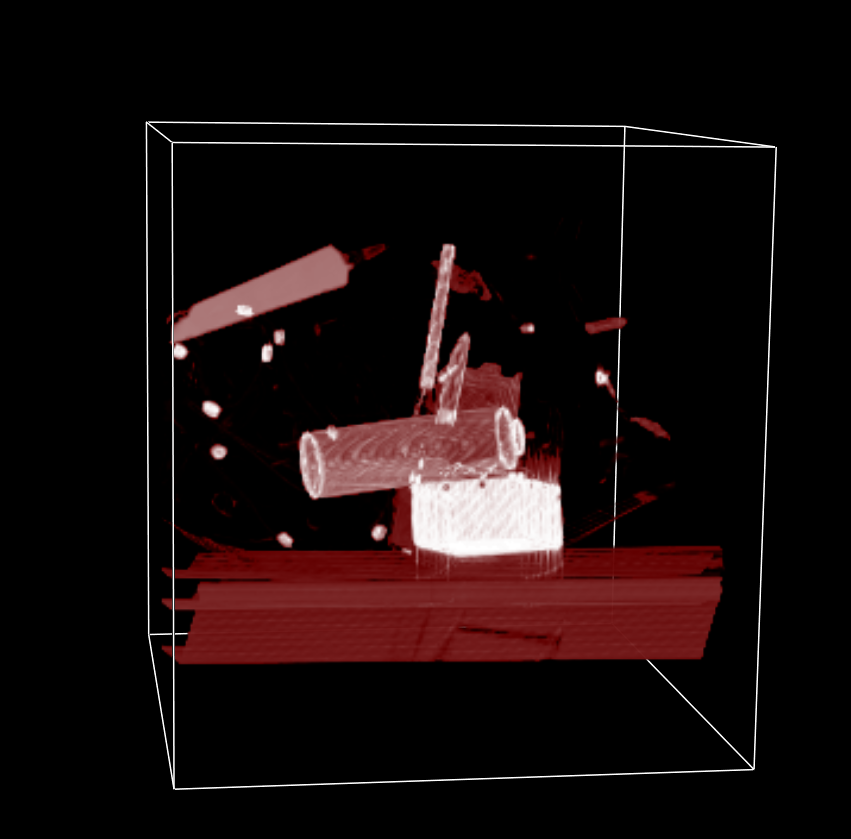
\includegraphics[width=0.5\textwidth]{MB.png}
  \caption{Resulting picture for backpack with MIP}
  \label{MB}
\end{figure}
\subsection{Bonsai}
This worked fine, we could see there was a tree. A picture is included in Figure \ref{MBon}.
\begin{figure}[!h]
  \centering
  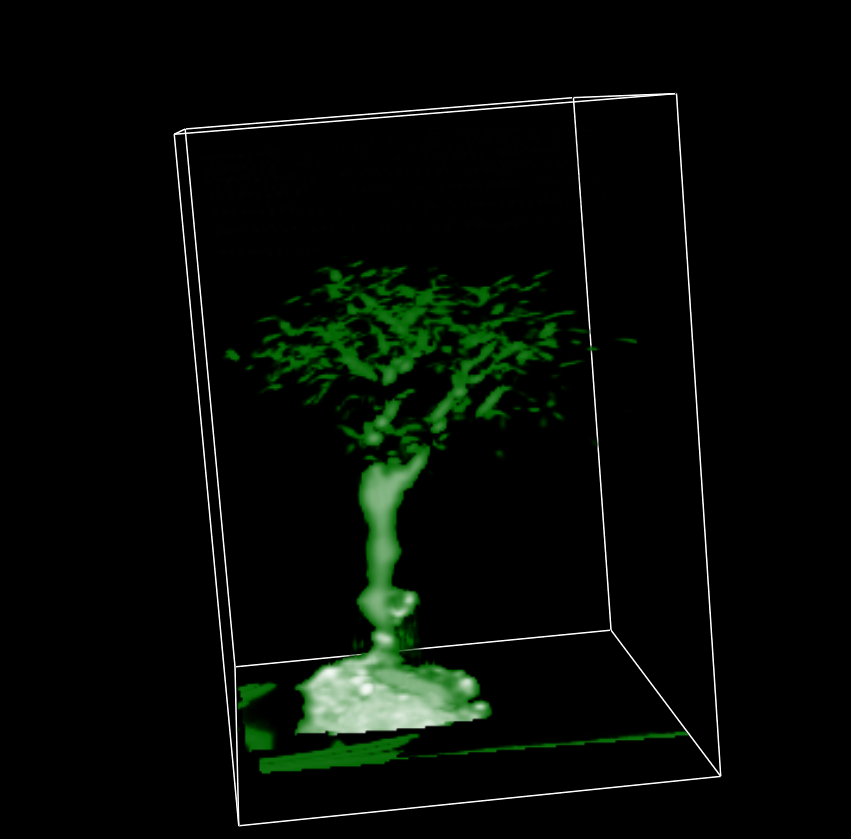
\includegraphics[width=0.5\textwidth]{MBon.png}
  \caption{Resulting picture for Bonsai with MIP}
  \label{MBon}
\end{figure}
\subsection{Carp}
This worked fantastic, we could see all the bones in the carp. A picture of the tail is included in Figure \ref{MCT}, the side is in Figure \ref{MCS}.
\begin{figure}[!h]
  \centering
  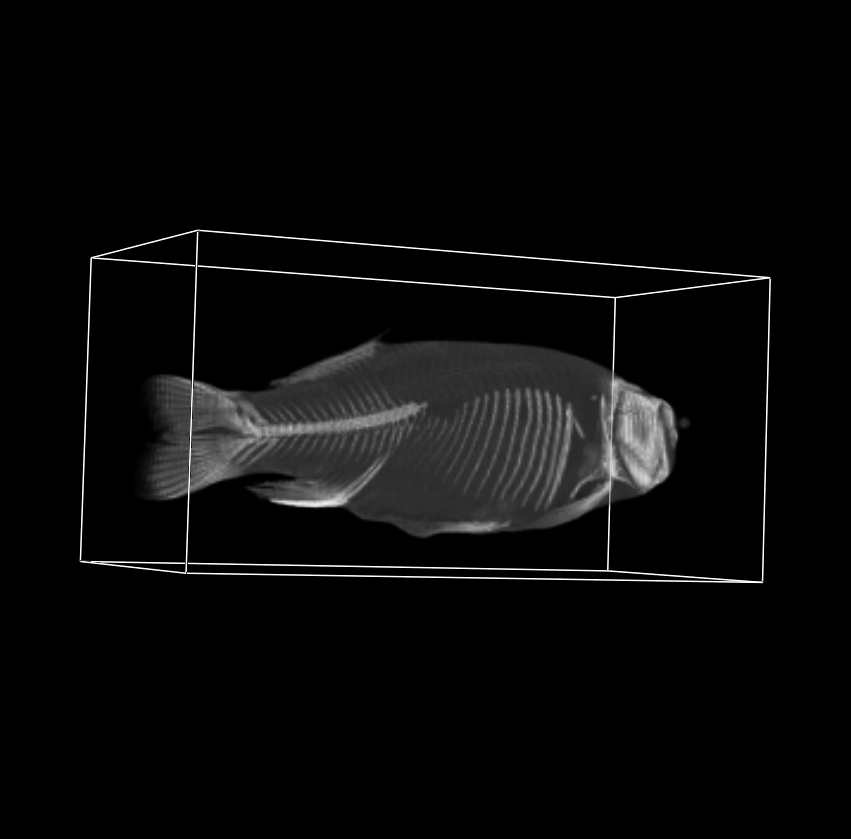
\includegraphics[width=0.5\textwidth]{MCT.png}
  \caption{Resulting picture for tail of the carp with MIP}
  \label{MCT}
\end{figure}
\begin{figure}[!h]
  \centering
  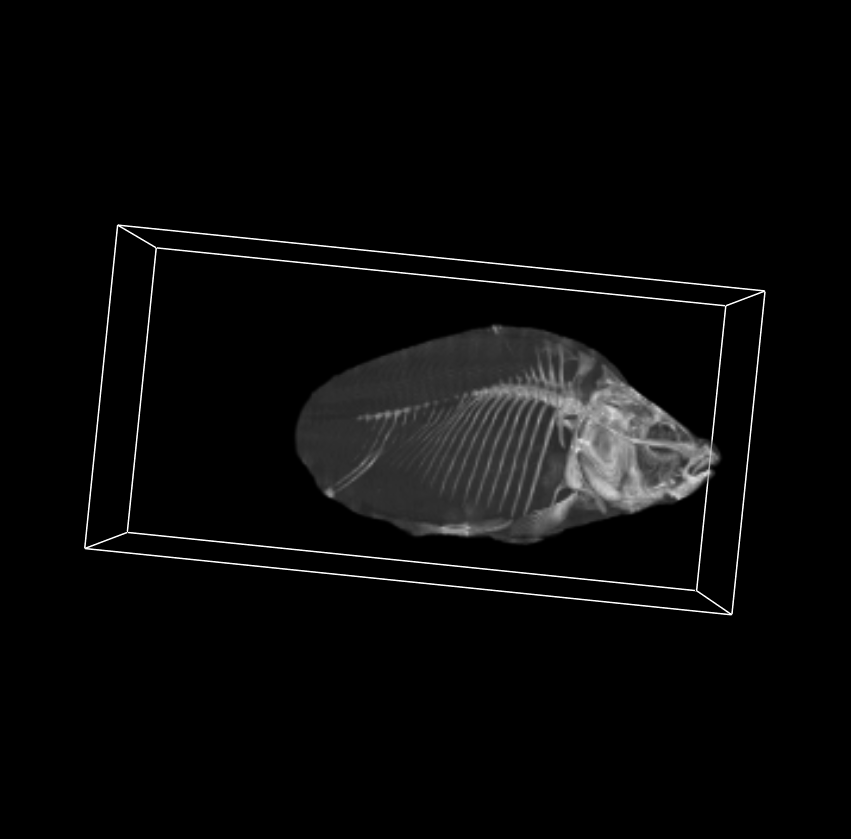
\includegraphics[width=0.5\textwidth]{MCS.png}
  \caption{Resulting picture for side of the carp with MIP}
  \label{MCS}
\end{figure}

\subsection{Orange}
This dataset leant itself to MIP too, we even were able to give the peel an orange color, while giving the inside a blue color. A picture is included in Figure \ref{MO}.
\begin{figure}[!h]
  \centering
  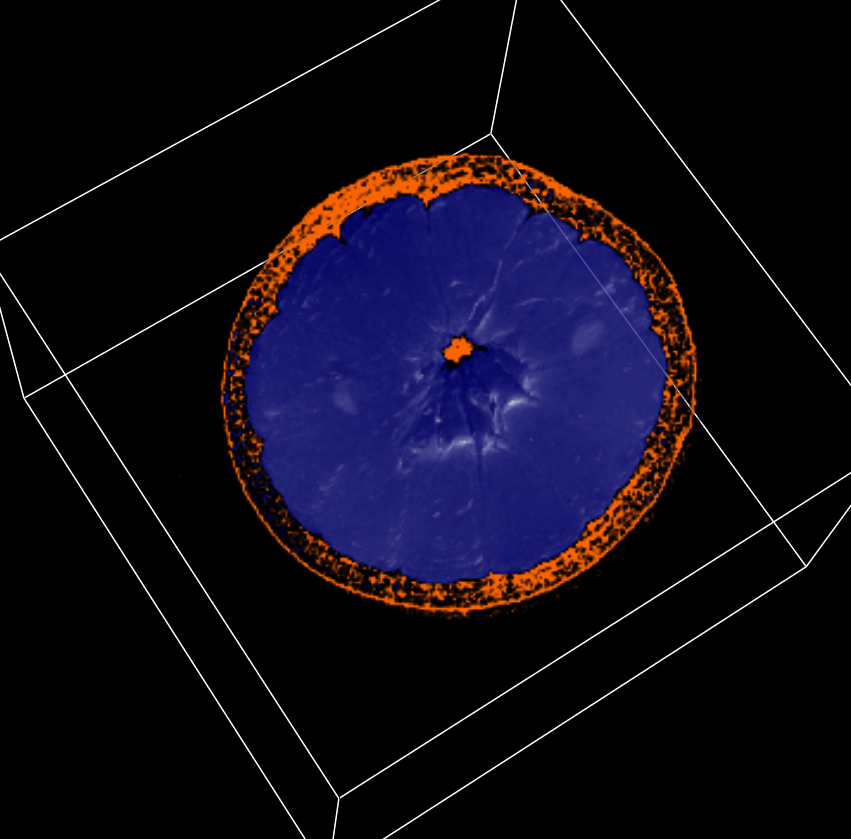
\includegraphics[width=0.5\textwidth]{MO.png}
  \caption{Resulting picture for orange with MIP}
  \label{MO}
\end{figure}

\subsection{Pig}
In this example we were able so show the coins in yellow and the pig in pink, also the hole is visible. A picture is included in Figure \ref{MP}.
\begin{figure}[!h]
  \centering
  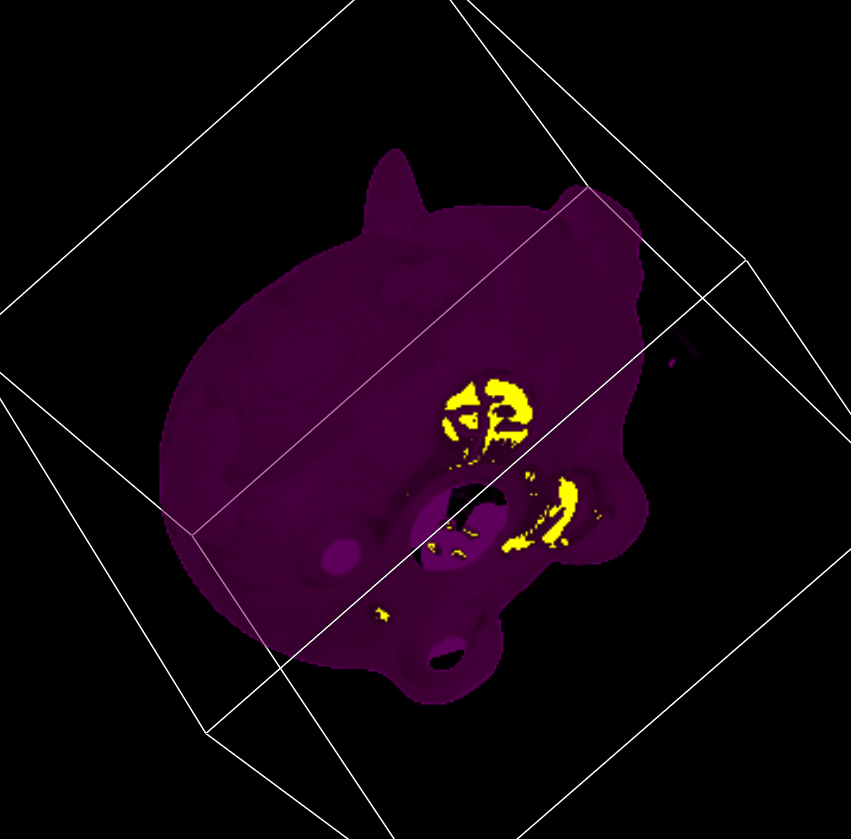
\includegraphics[width=0.5\textwidth]{MP.png}
  \caption{Resulting picture for pig with MIP}
  \label{MP}
\end{figure}

\subsection{Human}
Again a clear picture of a skeleton. A picture is included in Figure \ref{MH}.
\begin{figure}[!h]
  \centering
  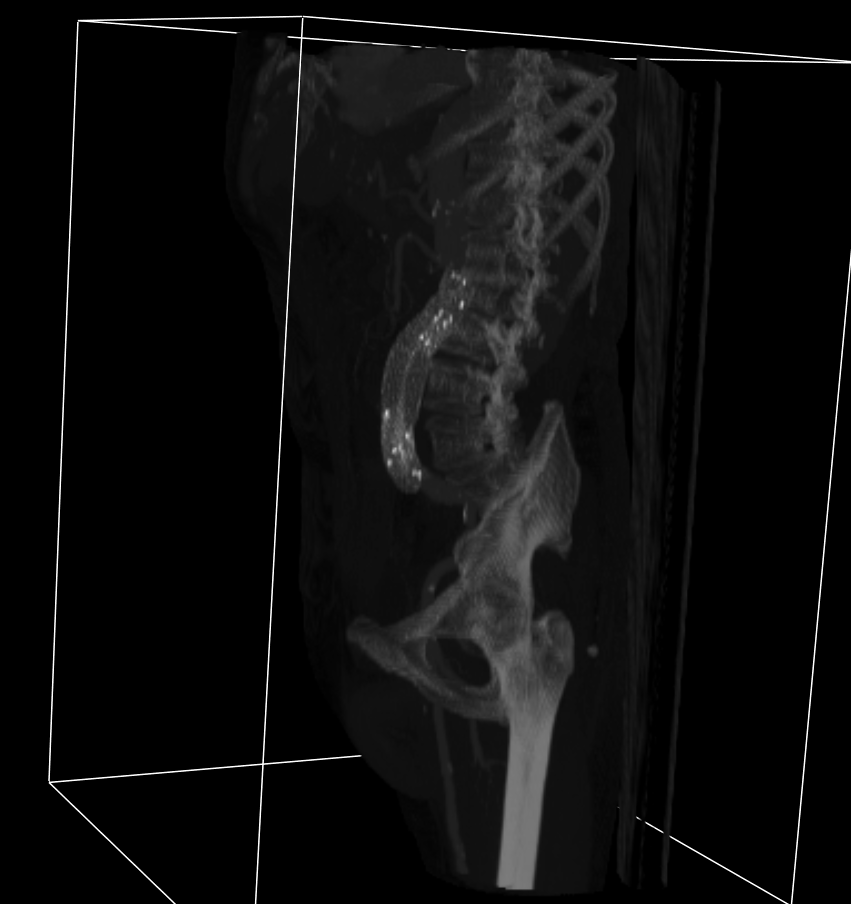
\includegraphics[width=0.5\textwidth]{MH.png}
  \caption{Resulting picture for human with MIP}
  \label{MH}
\end{figure}

\subsection{Tomato}
The tomato did not look very good as a picture because its quite homogeneous and quite similar to the orange, therefor we decided to omit a picture of it.

\subsection{Tooth}
The tooth data also produced nice results as can be seen in Figure \ref{MT}.
\begin{figure}[!h]
  \centering
  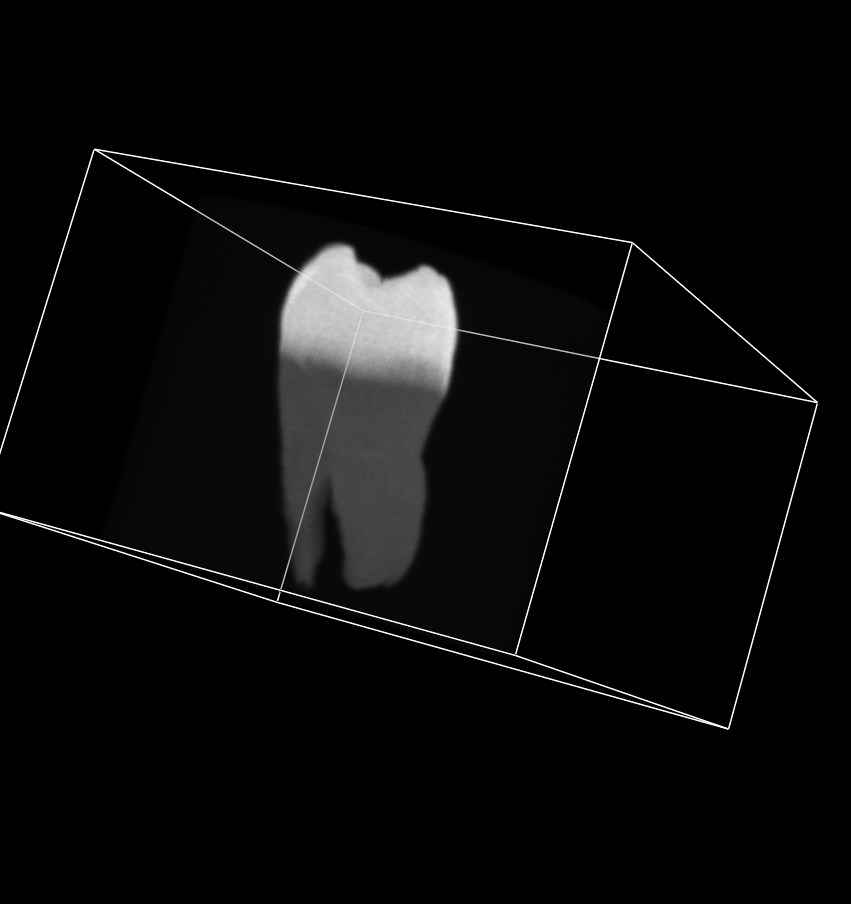
\includegraphics[width=0.5\textwidth]{MT.png}
  \caption{Resulting picture for tooth with MIP}
  \label{MT}
\end{figure}


\section{Transfer function}
In the transfer function we made at every sample $i$ the color $C_i$ is calculated, but there is also some color $C_{i-1}$ added behind it. This is done through the function $C_i = C(i)+ (1-\tau)C_{i-1}$.
 \subsection{Carp}
 Because its more dificult to find the correct colours we included a single picture, Figure \ref{hi}. It is nice to see the difference between the different tissues, we can see the green skin, the yellow brains, the red muscles and the grey bones.
 
 \section{Compositing}
 For compositing we implemented the standard formula given in slides of the course 2IV35 (Visualization) of the TU/e \cite{slideVis_m}. Compositing is a process where the values of all voxels along the ray are merged in such a way that one should be able to also look at the insides, where masses which are big will have a heavier impact on the picture then smaller masses. This can be remedied by setting the transfer function carefully but it could be that the transferfunction needs to be readjusted after rotating the picture, since now the ray has to traverse more or less of the material then it did previously.
 
 \subsection{Backpack}
 
 \subsection{Bonsai}
 
 \subsection{Carp}
 
 \subsection{Orange}
 
 \subsection{Pig}
 
 \subsection{Human}
 
 \subsection{Tomato}
 
 \subsection{Tooth}
 
 \newpage
 \section{Opacity weighting}
 Opacity weighting is implemented as discribed in a paper by Marc Levoy \cite{levoy_m}. Since there is a need for scaling the gradient magnitude, we implemented a scaling factor using a spinner, which can be used to scale the magnitude. We decided to use this method since it enables a person to have granulated control of the scaling which enables the selection of optimal values for making the borders visible. Opacity weighting remedies the problem of compositing since it voxels which define edges will be made much more visible then voxels in the middle of (homogenuous) masses. This enables more precise viewing of contents of volumes.
 
 \subsection{Backpack}
  \begin{figure}[H]
 
 \minipage{0.4\textwidth}
  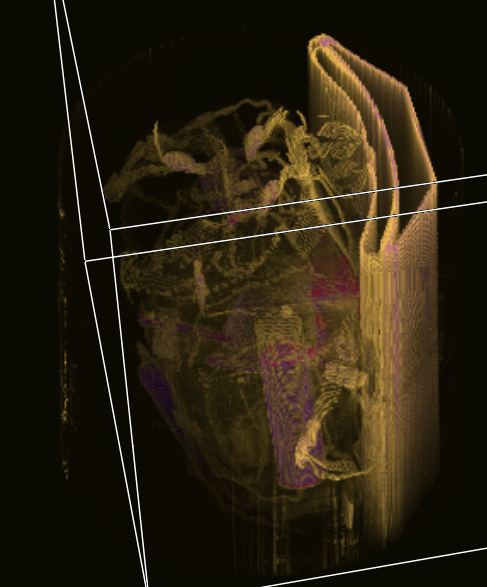
\includegraphics[width=\linewidth]{images/backpackOp}
  \caption{Backpack similar to composition}\label{toothOp}
\endminipage\hfill
\minipage{0.5\textwidth}
  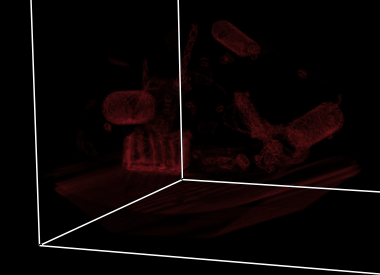
\includegraphics[width=\linewidth]{images/backpackOp2}
  \caption{Backpack with a look into the contents}\label{toothOp2}
\endminipage\hfill
 \end{figure}
 
 \subsection{Bonsai}
  \begin{figure}[h]
 \centering
 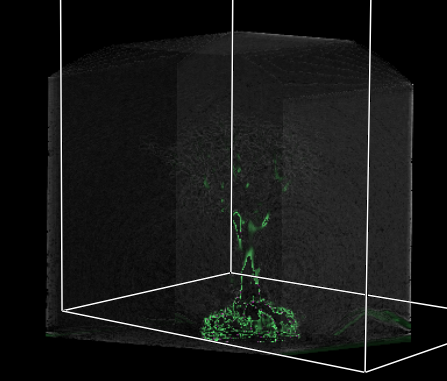
\includegraphics[scale=0.6]{images/bonsaiOp}
 \caption{The bonsai with the protective covering slightly visible}
 \label{carpOp}
 \end{figure}
 
 \subsection{Carp}
 When we applied opacity weighting to the carp dataset we could very quickly see that the carp was laid flat on some sheets which is presumable paper
 \begin{figure}[h]
 \centering
 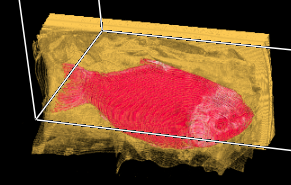
\includegraphics{images/carpOp}
 \caption{The carp with the protective surface visible}
 \label{carpOp}
 \end{figure}
 
 \subsection{Orange}
 \begin{figure}[H]
 \centering
 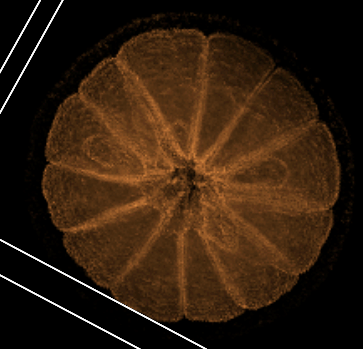
\includegraphics[scale=0.5]{images/orangeOp}
 \caption{}
 \label{orangeOp}
 \end{figure}
 
 \subsection{Pig}
 \begin{figure}[H]
 \centering
 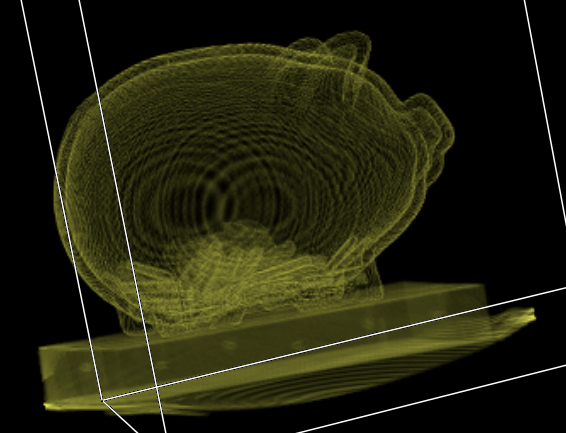
\includegraphics[scale=0.5]{images/pigOp}
 \caption{The piggybank with the coin contents made visible}
 \label{pigOp}
 \end{figure}
 
 \subsection{Human}
 \begin{figure}[H]
 \centering
 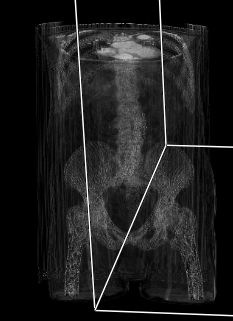
\includegraphics{images/bodyOp2}
 \caption{}
 \label{bodyOp}
 \end{figure}
 
 \subsection{Tomato}
 
 \begin{figure}[htb]
\minipage{0.32\textwidth}
  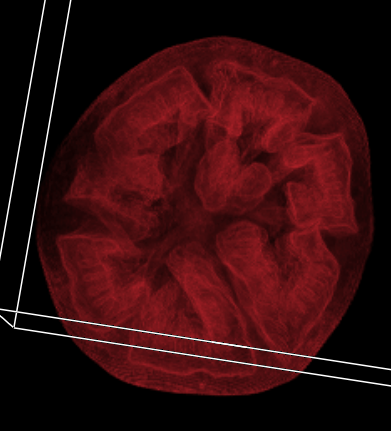
\includegraphics[width=\linewidth]{images/tomatoOp}
  \caption{Mixture of the pulp, the skind and water}\label{tomatoOp}
\endminipage\hfill
\minipage{0.32\textwidth}
  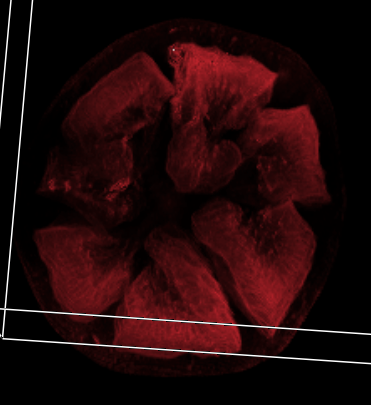
\includegraphics[width=\linewidth]{images/tomatoOp2}
  \caption{Only the pulp visible.}\label{tomateOp2}
\endminipage\hfill
\minipage{0.32\textwidth}%
  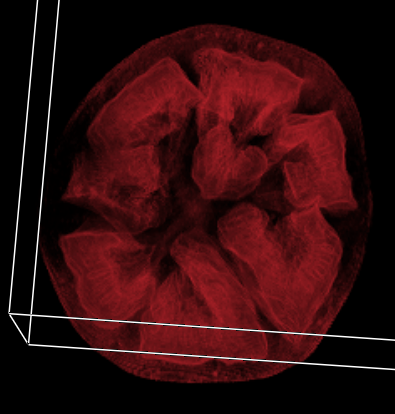
\includegraphics[width=\linewidth]{images/tomatoOp3}
  \caption{Tomato with some seeds visible}\label{tomatoOp3}
\endminipage
\end{figure}

 
 \subsection{Tooth}
 \begin{figure}[H]
 
 \minipage{0.4\textwidth}
  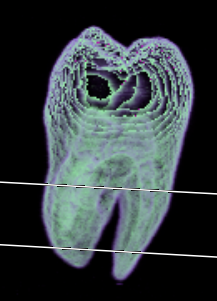
\includegraphics[width=\linewidth]{images/toothOp}
  \caption{The tooth with the root}\label{toothOp}
\endminipage\hfill
\minipage{0.5\textwidth}
  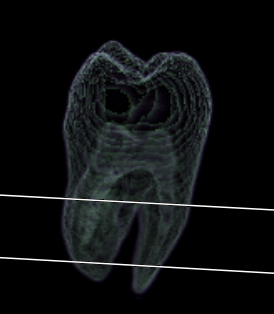
\includegraphics[width=\linewidth]{images/toothOp2}
  \caption{Tooth with a more visible root}\label{toothOp2}
\endminipage\hfill
 \end{figure}

\begin{figure}[!h]
  \centering
  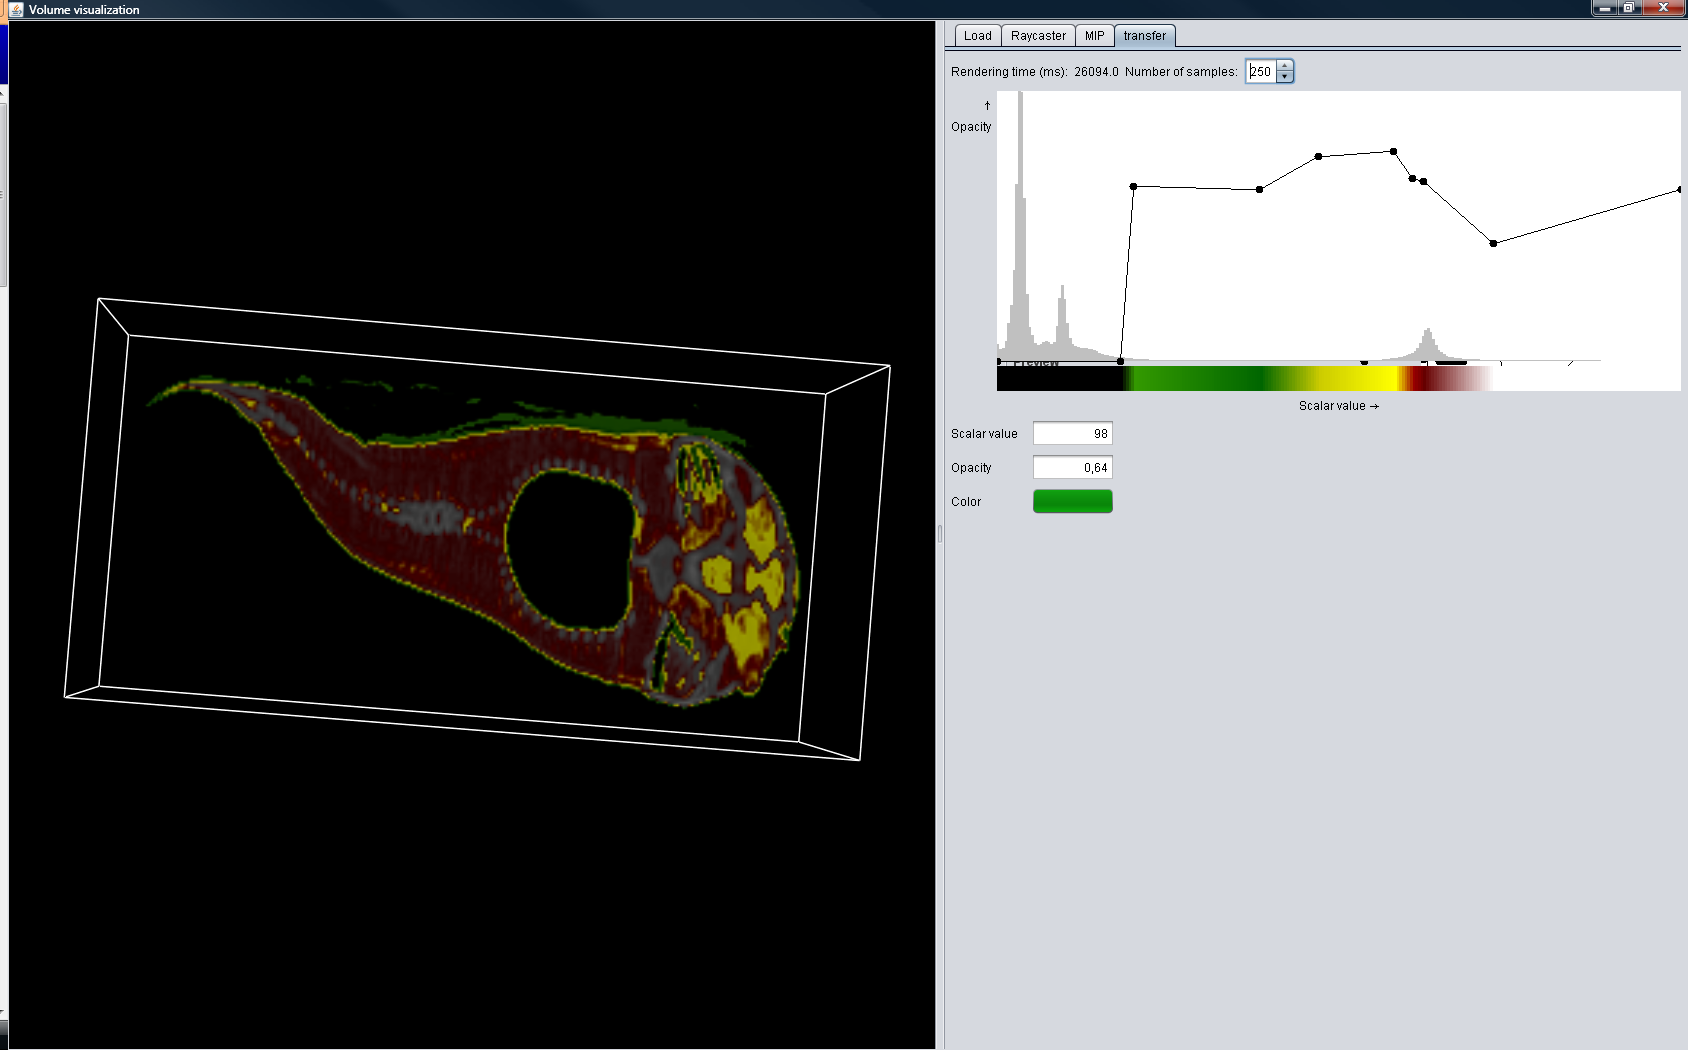
\includegraphics[width=1\textheight, angle=90]{hicarp.png}
  \caption{Resulting picture for the carp with transfer function}
  \label{hi}
\end{figure}
\end{document}


\begin{thebibliography}{9}
\bibitem{slideVis_m}
https://dlwpswbsp.tue.nl/120-2014/4d0982b89c664c579bd307b3c4ae82ca/Slides/4-spatial.pdf
\bibitem{levoy_m}
https://graphics.stanford.edu/papers/volume-cga88/volume.pdf
 \end{thebibliography}
\end{document}
